\hypertarget{vandeWiel_8c}{
\section{vande\-Wiel.c File Reference}
\label{vandeWiel_8c}\index{vandeWiel.c@{vandeWiel.c}}
}
{\tt \#include $<$R.h$>$}\par
{\tt \#include $<$Rmath.h$>$}\par
{\tt \#include $<$Rdefines.h$>$}\par


Include dependency graph for vande\-Wiel.c:\begin{figure}[H]
\begin{center}
\leavevmode
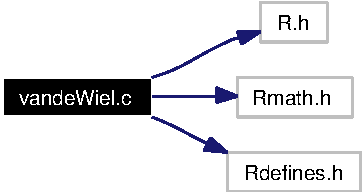
\includegraphics[width=104pt]{vandeWiel_8c__incl}
\end{center}
\end{figure}
\subsection*{Functions}
\begin{CompactItemize}
\item 
double \hyperlink{vandeWiel_8c_a0}{binomi} (int m, int n)
\item 
\hyperlink{structcelW}{cel\-W} $\ast$$\ast$ \hyperlink{vandeWiel_8c_a1}{reserve\-W} (int a, int b)
\item 
void \hyperlink{vandeWiel_8c_a2}{Free\-W} (int a, \hyperlink{structcelW}{cel\-W} $\ast$$\ast$W)
\item 
void \hyperlink{vandeWiel_8c_a3}{init\-W} (int a, int b, \hyperlink{structcelW}{cel\-W} $\ast$$\ast$W)
\item 
void \hyperlink{vandeWiel_8c_a4}{mult} (\hyperlink{structcelW}{cel\-W} $\ast$tem, int a, int b, int rank, double $\ast$rs)
\item 
void \hyperlink{vandeWiel_8c_a5}{plus} (\hyperlink{structcelW}{cel\-W} $\ast$$\ast$W, \hyperlink{structcelW}{cel\-W} $\ast$tempie, int a, int b)
\item 
void \hyperlink{vandeWiel_8c_a6}{mymergesort} (\hyperlink{structcelW}{cel\-W} temptw, long tijd)
\item 
void \hyperlink{vandeWiel_8c_a7}{fillcell} (\hyperlink{structcelW}{cel\-W} $\ast$$\ast$W, int i1, int j1, int r, double $\ast$rs)
\item 
void \hyperlink{vandeWiel_8c_a8}{mirror\-W} (\hyperlink{structcelW}{cel\-W} $\ast$$\ast$W, int ce, int bep, int start, double $\ast$rs)
\item 
void \hyperlink{vandeWiel_8c_a9}{make\-W} (\hyperlink{structcelW}{cel\-W} $\ast$$\ast$W, int a, int b, int start, double $\ast$rs)
\item 
void \hyperlink{vandeWiel_8c_a10}{cumulcoef} (\hyperlink{structcelW}{cel\-W} $\ast$$\ast$W, int i1, int j1)
\item 
double \hyperlink{vandeWiel_8c_a11}{numbersmall} (int c, int b, double ob, \hyperlink{structcelW}{cel\-W} $\ast$$\ast$W1, \hyperlink{structcelW}{cel\-W} $\ast$$\ast$W2)
\item 
SEXP \hyperlink{vandeWiel_8c_a12}{R\_\-split\_\-up\_\-2sample} (SEXP scores, SEXP m, SEXP obs)
\end{CompactItemize}


\subsection{Detailed Description}
Exact Distribution of Two-Sample Permutation Tests van de Wiel split-up Algorithm

Author: Mark van de Wiel (2001-2005) $<$\href{mailto:m.a.v.d.wiel@TUE.nl}{\tt m.a.v.d.wiel@TUE.nl}$>$ with modifications for R by Torsten Hothorn $<$\href{mailto:Torsten.Hothorn@R-project.org}{\tt Torsten.Hothorn@R-project.org}$>$

\begin{Desc}
\item[Author:]\begin{Desc}
\item[Author]hothorn \end{Desc}
\end{Desc}
\begin{Desc}
\item[Date:]\begin{Desc}
\item[Date]2005/07/28 15:04:29 \end{Desc}
\end{Desc}


Definition in file \hyperlink{vandeWiel_8c-source}{vande\-Wiel.c}.

\subsection{Function Documentation}
\hypertarget{vandeWiel_8c_a0}{
\index{vandeWiel.c@{vande\-Wiel.c}!binomi@{binomi}}
\index{binomi@{binomi}!vandeWiel.c@{vande\-Wiel.c}}
\subsubsection[binomi]{\setlength{\rightskip}{0pt plus 5cm}double binomi (int {\em m}, int {\em n})}}
\label{vandeWiel_8c_a0}




Definition at line 37 of file vande\-Wiel.c.

Referenced by R\_\-split\_\-up\_\-2sample(), and reserve\-W().\hypertarget{vandeWiel_8c_a10}{
\index{vandeWiel.c@{vande\-Wiel.c}!cumulcoef@{cumulcoef}}
\index{cumulcoef@{cumulcoef}!vandeWiel.c@{vande\-Wiel.c}}
\subsubsection[cumulcoef]{\setlength{\rightskip}{0pt plus 5cm}void cumulcoef (\hyperlink{structcelW}{cel\-W} $\ast$$\ast$ {\em W}, int {\em i1}, int {\em j1})}}
\label{vandeWiel_8c_a10}




Definition at line 316 of file vande\-Wiel.c.

References cel\-W::c, and cel\-W::length.

Referenced by R\_\-split\_\-up\_\-2sample().\hypertarget{vandeWiel_8c_a7}{
\index{vandeWiel.c@{vande\-Wiel.c}!fillcell@{fillcell}}
\index{fillcell@{fillcell}!vandeWiel.c@{vande\-Wiel.c}}
\subsubsection[fillcell]{\setlength{\rightskip}{0pt plus 5cm}void fillcell (\hyperlink{structcelW}{cel\-W} $\ast$$\ast$ {\em W}, int {\em i1}, int {\em j1}, int {\em r}, double $\ast$ {\em rs})}}
\label{vandeWiel_8c_a7}




Definition at line 211 of file vande\-Wiel.c.

References cel\-W::c, cel\-W::length, mult(), mymergesort(), plus(), and cel\-W::x.

Referenced by make\-W().

Here is the call graph for this function:\begin{figure}[H]
\begin{center}
\leavevmode
\includegraphics[width=95pt]{vandeWiel_8c_a7_cgraph}
\end{center}
\end{figure}
\hypertarget{vandeWiel_8c_a2}{
\index{vandeWiel.c@{vande\-Wiel.c}!FreeW@{FreeW}}
\index{FreeW@{FreeW}!vandeWiel.c@{vande\-Wiel.c}}
\subsubsection[FreeW]{\setlength{\rightskip}{0pt plus 5cm}void Free\-W (int {\em a}, \hyperlink{structcelW}{cel\-W} $\ast$$\ast$ {\em W})}}
\label{vandeWiel_8c_a2}




Definition at line 81 of file vande\-Wiel.c.

Referenced by R\_\-split\_\-up\_\-2sample().\hypertarget{vandeWiel_8c_a3}{
\index{vandeWiel.c@{vande\-Wiel.c}!initW@{initW}}
\index{initW@{initW}!vandeWiel.c@{vande\-Wiel.c}}
\subsubsection[initW]{\setlength{\rightskip}{0pt plus 5cm}void init\-W (int {\em a}, int {\em b}, \hyperlink{structcelW}{cel\-W} $\ast$$\ast$ {\em W})}}
\label{vandeWiel_8c_a3}




Definition at line 91 of file vande\-Wiel.c.

References cel\-W::c, cel\-W::length, and cel\-W::x.

Referenced by R\_\-split\_\-up\_\-2sample().\hypertarget{vandeWiel_8c_a9}{
\index{vandeWiel.c@{vande\-Wiel.c}!makeW@{makeW}}
\index{makeW@{makeW}!vandeWiel.c@{vande\-Wiel.c}}
\subsubsection[makeW]{\setlength{\rightskip}{0pt plus 5cm}void make\-W (\hyperlink{structcelW}{cel\-W} $\ast$$\ast$ {\em W}, int {\em a}, int {\em b}, int {\em start}, double $\ast$ {\em rs})}}
\label{vandeWiel_8c_a9}




Definition at line 281 of file vande\-Wiel.c.

References fillcell(), and mirror\-W().

Referenced by R\_\-split\_\-up\_\-2sample().

Here is the call graph for this function:\begin{figure}[H]
\begin{center}
\leavevmode
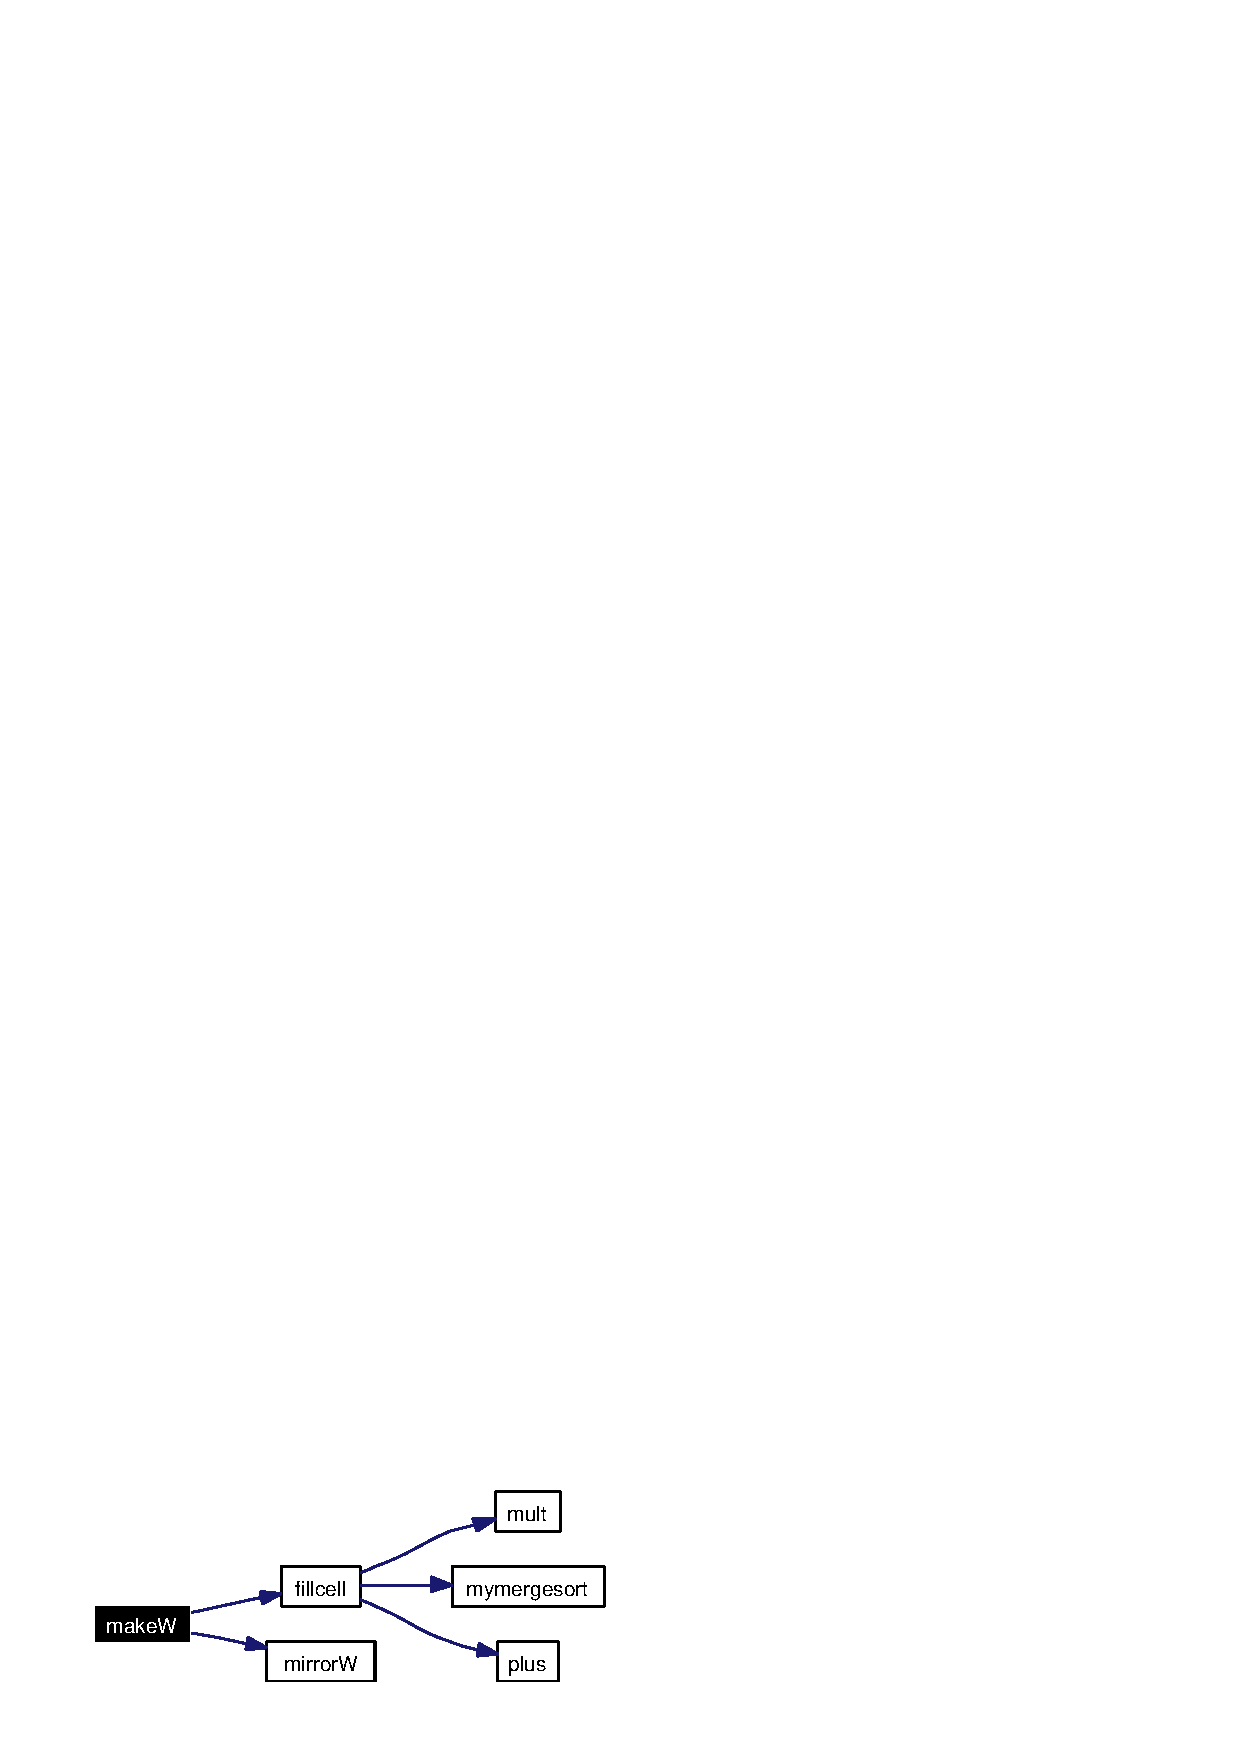
\includegraphics[width=144pt]{vandeWiel_8c_a9_cgraph}
\end{center}
\end{figure}
\hypertarget{vandeWiel_8c_a8}{
\index{vandeWiel.c@{vande\-Wiel.c}!mirrorW@{mirrorW}}
\index{mirrorW@{mirrorW}!vandeWiel.c@{vande\-Wiel.c}}
\subsubsection[mirrorW]{\setlength{\rightskip}{0pt plus 5cm}void mirror\-W (\hyperlink{structcelW}{cel\-W} $\ast$$\ast$ {\em W}, int {\em ce}, int {\em bep}, int {\em start}, double $\ast$ {\em rs})}}
\label{vandeWiel_8c_a8}




Definition at line 257 of file vande\-Wiel.c.

References cel\-W::c, cel\-W::length, and cel\-W::x.

Referenced by make\-W().\hypertarget{vandeWiel_8c_a4}{
\index{vandeWiel.c@{vande\-Wiel.c}!mult@{mult}}
\index{mult@{mult}!vandeWiel.c@{vande\-Wiel.c}}
\subsubsection[mult]{\setlength{\rightskip}{0pt plus 5cm}void mult (\hyperlink{structcelW}{cel\-W} $\ast$ {\em tem}, int {\em a}, int {\em b}, int {\em rank}, double $\ast$ {\em rs})}}
\label{vandeWiel_8c_a4}




Definition at line 106 of file vande\-Wiel.c.

References cel\-W::x.

Referenced by fillcell().\hypertarget{vandeWiel_8c_a6}{
\index{vandeWiel.c@{vande\-Wiel.c}!mymergesort@{mymergesort}}
\index{mymergesort@{mymergesort}!vandeWiel.c@{vande\-Wiel.c}}
\subsubsection[mymergesort]{\setlength{\rightskip}{0pt plus 5cm}void mymergesort (\hyperlink{structcelW}{cel\-W} {\em temptw}, long {\em tijd})}}
\label{vandeWiel_8c_a6}




Definition at line 159 of file vande\-Wiel.c.

References cel\-W::c, cel\-W::length, and cel\-W::x.

Referenced by fillcell().\hypertarget{vandeWiel_8c_a11}{
\index{vandeWiel.c@{vande\-Wiel.c}!numbersmall@{numbersmall}}
\index{numbersmall@{numbersmall}!vandeWiel.c@{vande\-Wiel.c}}
\subsubsection[numbersmall]{\setlength{\rightskip}{0pt plus 5cm}double numbersmall (int {\em c}, int {\em b}, double {\em ob}, \hyperlink{structcelW}{cel\-W} $\ast$$\ast$ {\em W1}, \hyperlink{structcelW}{cel\-W} $\ast$$\ast$ {\em W2})}}
\label{vandeWiel_8c_a11}




Definition at line 335 of file vande\-Wiel.c.

References cel\-W::c, and cel\-W::length.

Referenced by R\_\-split\_\-up\_\-2sample().\hypertarget{vandeWiel_8c_a5}{
\index{vandeWiel.c@{vande\-Wiel.c}!plus@{plus}}
\index{plus@{plus}!vandeWiel.c@{vande\-Wiel.c}}
\subsubsection[plus]{\setlength{\rightskip}{0pt plus 5cm}void plus (\hyperlink{structcelW}{cel\-W} $\ast$$\ast$ {\em W}, \hyperlink{structcelW}{cel\-W} $\ast$ {\em tempie}, int {\em a}, int {\em b})}}
\label{vandeWiel_8c_a5}




Definition at line 120 of file vande\-Wiel.c.

References cel\-W::c, cel\-W::length, and cel\-W::x.

Referenced by fillcell().\hypertarget{vandeWiel_8c_a12}{
\index{vandeWiel.c@{vande\-Wiel.c}!R_split_up_2sample@{R\_\-split\_\-up\_\-2sample}}
\index{R_split_up_2sample@{R\_\-split\_\-up\_\-2sample}!vandeWiel.c@{vande\-Wiel.c}}
\subsubsection[R\_\-split\_\-up\_\-2sample]{\setlength{\rightskip}{0pt plus 5cm}SEXP R\_\-split\_\-up\_\-2sample (SEXP {\em scores}, SEXP {\em m}, SEXP {\em obs})}}
\label{vandeWiel_8c_a12}




Definition at line 375 of file vande\-Wiel.c.

References binomi(), cumulcoef(), Free\-W(), init\-W(), make\-W(), numbersmall(), and reserve\-W().

Here is the call graph for this function:\begin{figure}[H]
\begin{center}
\leavevmode
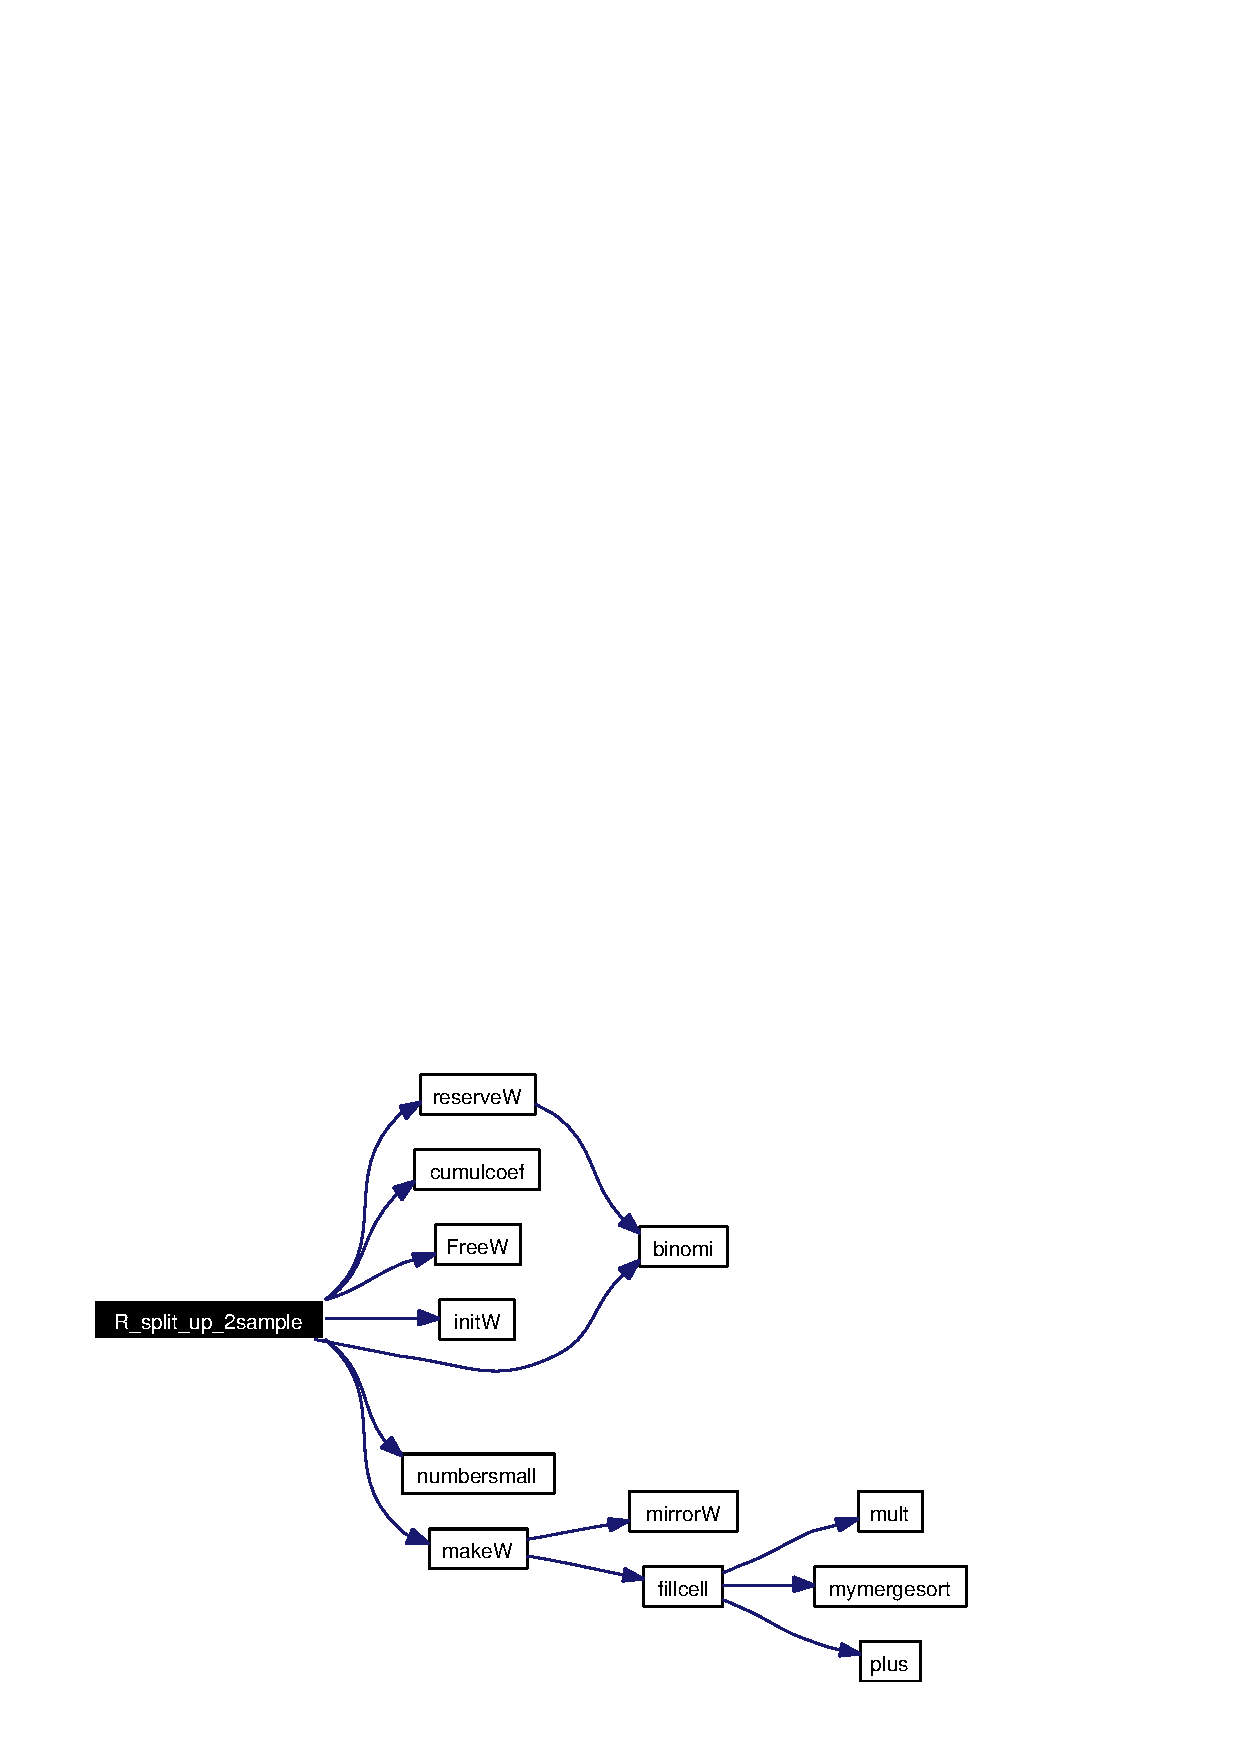
\includegraphics[width=227pt]{vandeWiel_8c_a12_cgraph}
\end{center}
\end{figure}
\hypertarget{vandeWiel_8c_a1}{
\index{vandeWiel.c@{vande\-Wiel.c}!reserveW@{reserveW}}
\index{reserveW@{reserveW}!vandeWiel.c@{vande\-Wiel.c}}
\subsubsection[reserveW]{\setlength{\rightskip}{0pt plus 5cm}\hyperlink{structcelW}{cel\-W}$\ast$$\ast$ reserve\-W (int {\em a}, int {\em b})}}
\label{vandeWiel_8c_a1}




Definition at line 51 of file vande\-Wiel.c.

References binomi(), cel\-W::c, and cel\-W::x.

Referenced by R\_\-split\_\-up\_\-2sample().

Here is the call graph for this function:\begin{figure}[H]
\begin{center}
\leavevmode
\includegraphics[width=89pt]{vandeWiel_8c_a1_cgraph}
\end{center}
\end{figure}
